% Options for packages loaded elsewhere
% Options for packages loaded elsewhere
\PassOptionsToPackage{unicode}{hyperref}
\PassOptionsToPackage{hyphens}{url}
\PassOptionsToPackage{dvipsnames,svgnames,x11names}{xcolor}
%
\documentclass[
  letterpaper,
  DIV=11,
  numbers=noendperiod]{scrartcl}
\usepackage{xcolor}
\usepackage{amsmath,amssymb}
\setcounter{secnumdepth}{-\maxdimen} % remove section numbering
\usepackage{iftex}
\ifPDFTeX
  \usepackage[T1]{fontenc}
  \usepackage[utf8]{inputenc}
  \usepackage{textcomp} % provide euro and other symbols
\else % if luatex or xetex
  \usepackage{unicode-math} % this also loads fontspec
  \defaultfontfeatures{Scale=MatchLowercase}
  \defaultfontfeatures[\rmfamily]{Ligatures=TeX,Scale=1}
\fi
\usepackage{lmodern}
\ifPDFTeX\else
  % xetex/luatex font selection
\fi
% Use upquote if available, for straight quotes in verbatim environments
\IfFileExists{upquote.sty}{\usepackage{upquote}}{}
\IfFileExists{microtype.sty}{% use microtype if available
  \usepackage[]{microtype}
  \UseMicrotypeSet[protrusion]{basicmath} % disable protrusion for tt fonts
}{}
\makeatletter
\@ifundefined{KOMAClassName}{% if non-KOMA class
  \IfFileExists{parskip.sty}{%
    \usepackage{parskip}
  }{% else
    \setlength{\parindent}{0pt}
    \setlength{\parskip}{6pt plus 2pt minus 1pt}}
}{% if KOMA class
  \KOMAoptions{parskip=half}}
\makeatother
% Make \paragraph and \subparagraph free-standing
\makeatletter
\ifx\paragraph\undefined\else
  \let\oldparagraph\paragraph
  \renewcommand{\paragraph}{
    \@ifstar
      \xxxParagraphStar
      \xxxParagraphNoStar
  }
  \newcommand{\xxxParagraphStar}[1]{\oldparagraph*{#1}\mbox{}}
  \newcommand{\xxxParagraphNoStar}[1]{\oldparagraph{#1}\mbox{}}
\fi
\ifx\subparagraph\undefined\else
  \let\oldsubparagraph\subparagraph
  \renewcommand{\subparagraph}{
    \@ifstar
      \xxxSubParagraphStar
      \xxxSubParagraphNoStar
  }
  \newcommand{\xxxSubParagraphStar}[1]{\oldsubparagraph*{#1}\mbox{}}
  \newcommand{\xxxSubParagraphNoStar}[1]{\oldsubparagraph{#1}\mbox{}}
\fi
\makeatother


\usepackage{longtable,booktabs,array}
\usepackage{calc} % for calculating minipage widths
% Correct order of tables after \paragraph or \subparagraph
\usepackage{etoolbox}
\makeatletter
\patchcmd\longtable{\par}{\if@noskipsec\mbox{}\fi\par}{}{}
\makeatother
% Allow footnotes in longtable head/foot
\IfFileExists{footnotehyper.sty}{\usepackage{footnotehyper}}{\usepackage{footnote}}
\makesavenoteenv{longtable}
\usepackage{graphicx}
\makeatletter
\newsavebox\pandoc@box
\newcommand*\pandocbounded[1]{% scales image to fit in text height/width
  \sbox\pandoc@box{#1}%
  \Gscale@div\@tempa{\textheight}{\dimexpr\ht\pandoc@box+\dp\pandoc@box\relax}%
  \Gscale@div\@tempb{\linewidth}{\wd\pandoc@box}%
  \ifdim\@tempb\p@<\@tempa\p@\let\@tempa\@tempb\fi% select the smaller of both
  \ifdim\@tempa\p@<\p@\scalebox{\@tempa}{\usebox\pandoc@box}%
  \else\usebox{\pandoc@box}%
  \fi%
}
% Set default figure placement to htbp
\def\fps@figure{htbp}
\makeatother





\setlength{\emergencystretch}{3em} % prevent overfull lines

\providecommand{\tightlist}{%
  \setlength{\itemsep}{0pt}\setlength{\parskip}{0pt}}



 


\KOMAoption{captions}{tableheading}
\makeatletter
\@ifpackageloaded{caption}{}{\usepackage{caption}}
\AtBeginDocument{%
\ifdefined\contentsname
  \renewcommand*\contentsname{Table of contents}
\else
  \newcommand\contentsname{Table of contents}
\fi
\ifdefined\listfigurename
  \renewcommand*\listfigurename{List of Figures}
\else
  \newcommand\listfigurename{List of Figures}
\fi
\ifdefined\listtablename
  \renewcommand*\listtablename{List of Tables}
\else
  \newcommand\listtablename{List of Tables}
\fi
\ifdefined\figurename
  \renewcommand*\figurename{Figure}
\else
  \newcommand\figurename{Figure}
\fi
\ifdefined\tablename
  \renewcommand*\tablename{Table}
\else
  \newcommand\tablename{Table}
\fi
}
\@ifpackageloaded{float}{}{\usepackage{float}}
\floatstyle{ruled}
\@ifundefined{c@chapter}{\newfloat{codelisting}{h}{lop}}{\newfloat{codelisting}{h}{lop}[chapter]}
\floatname{codelisting}{Listing}
\newcommand*\listoflistings{\listof{codelisting}{List of Listings}}
\makeatother
\makeatletter
\makeatother
\makeatletter
\@ifpackageloaded{caption}{}{\usepackage{caption}}
\@ifpackageloaded{subcaption}{}{\usepackage{subcaption}}
\makeatother
\usepackage{bookmark}
\IfFileExists{xurl.sty}{\usepackage{xurl}}{} % add URL line breaks if available
\urlstyle{same}
\hypersetup{
  pdftitle={Digital Tools},
  colorlinks=true,
  linkcolor={blue},
  filecolor={Maroon},
  citecolor={Blue},
  urlcolor={Blue},
  pdfcreator={LaTeX via pandoc}}


\title{Digital Tools}
\author{}
\date{}
\begin{document}
\maketitle


\subsection{Module Overview}\label{module-overview}

\begin{itemize}
\tightlist
\item
  \textbf{Module:} EDS-M1 - Digital Tools
\item
  \textbf{Course:} Essential Digital Skills (EDS)
\item
  \textbf{Audience:} Early Career Researchers (PhD, Postdoc)\\
\item
  \textbf{Duration:} \textasciitilde40 minutes directed teaching (+4
  exercises)
\end{itemize}

\begin{center}\rule{0.5\linewidth}{0.5pt}\end{center}

\subsection{💡 Learning Outcomes}\label{learning-outcomes}

\begin{itemize}
\tightlist
\item
  Navigate core UoN digital ecosystem
\item
  Apply digital best practices in collaboration \& file organisation
\item
  Manage your research identity
\item
  Identify essential practices for secure research
\end{itemize}

\begin{center}\rule{0.5\linewidth}{0.5pt}\end{center}

\subsection{❓ Questions}\label{questions}

\begin{enumerate}
\def\labelenumi{\arabic{enumi}.}
\tightlist
\item
  What basic data tools I need to do research at UoN?
\item
  How to I maintain a consistent online researcher identity?
\item
  What digital tools may I need to support my research aims?\\
\end{enumerate}

\subsection{Structure \& Agenda}\label{structure-agenda}

\begin{enumerate}
\def\labelenumi{\arabic{enumi}.}
\tightlist
\item
  Introduction to the Digital Skills Programme (\textasciitilde10+10
  min)\\
\item
  Institutional Systems for Digital Research (\textasciitilde10+10
  min)\\
\item
  Research Identity and Profiles (\textasciitilde10+10 min)\\
\item
  Digital Security \& Good Practice (\textasciitilde10+10min)
\end{enumerate}

\begin{quote}
🔧 4 Activities spaced every 10 minutes.
\end{quote}

\section{Introduction to the Digital Skills
Programme}\label{introduction-to-the-digital-skills-programme}

\begin{center}
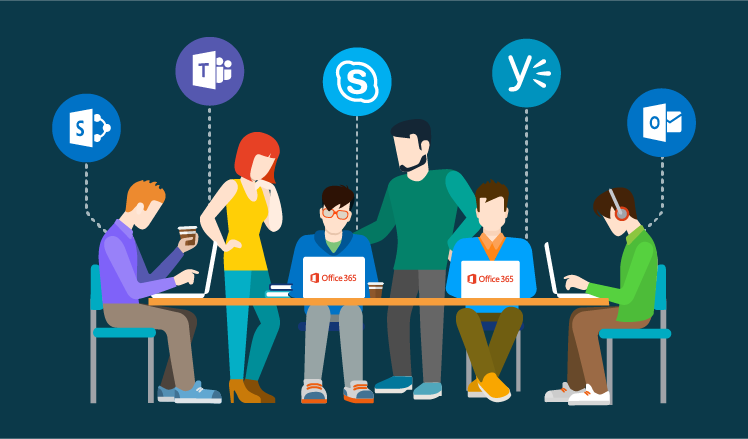
\includegraphics[width=5.20833in,height=\textheight,keepaspectratio]{fig/office365.png}
\end{center}

\subsection{What is DS?}\label{what-is-ds}

The \textbf{Digital Skills} programme equips researchers with the
competencies required for modern, data-driven scholarship. it focuses on
four interconnected themes:

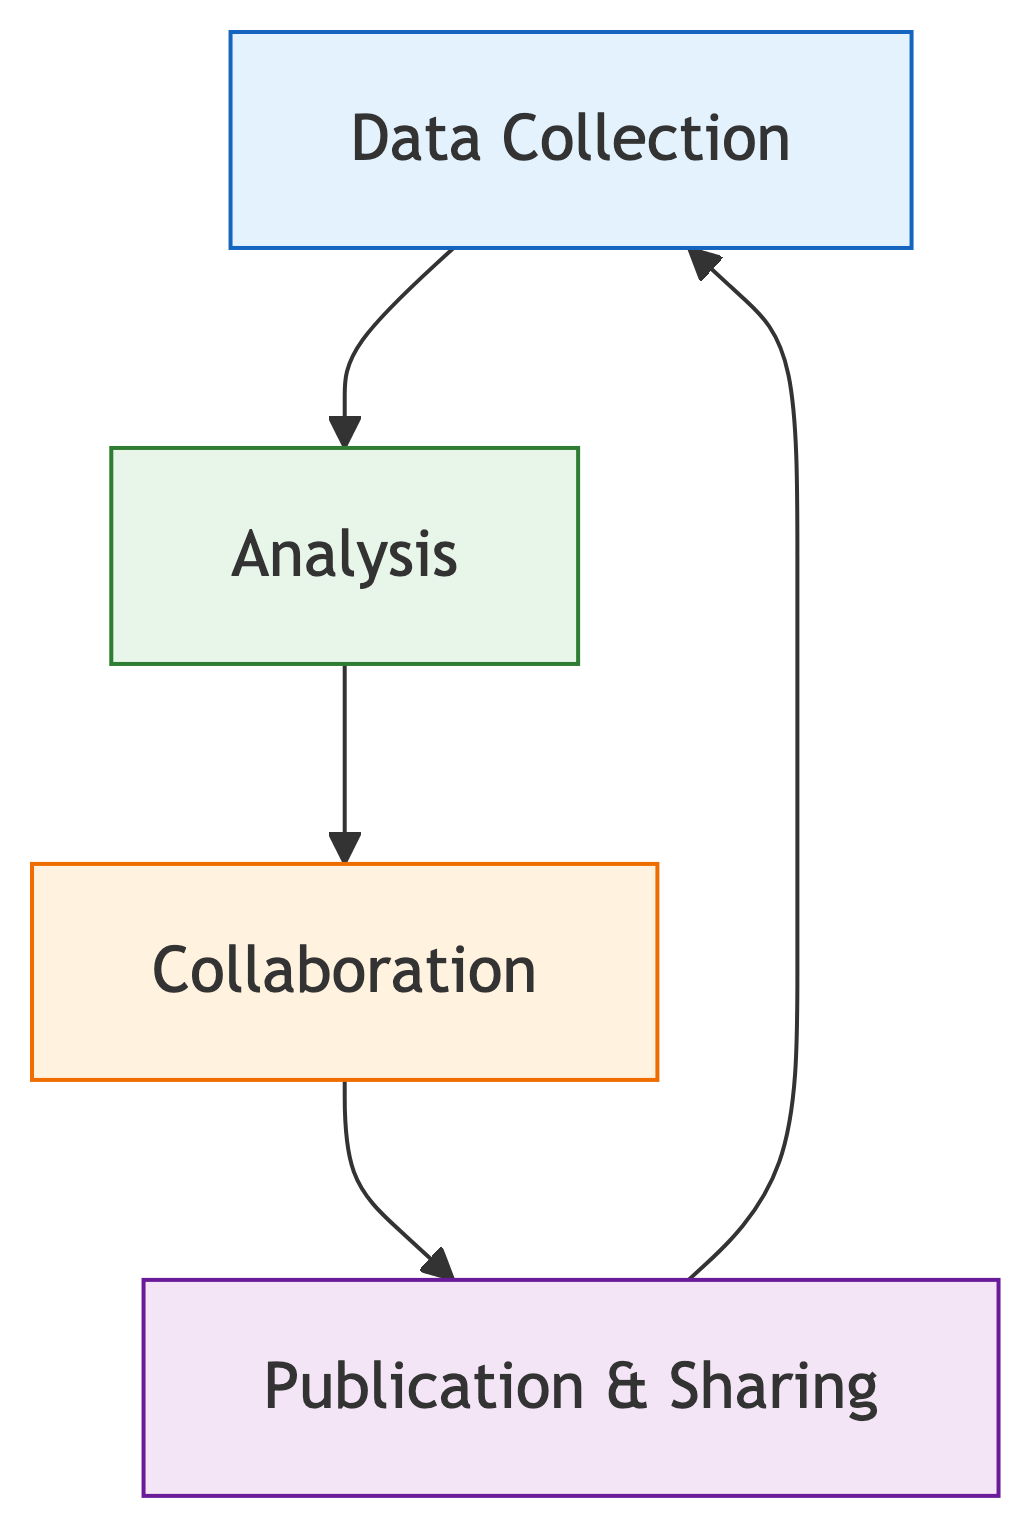
\includegraphics[width=8.74in,height=1.09in]{01-digital_tools_files/figure-latex/mermaid-figure-1.png}

\begin{quote}
💡 \emph{Digital collaboration, data management, coding, and
reproducibility form the foundation of digital research practice.}
\end{quote}

\subsection{Beyond Tools}\label{beyond-tools}

The programme is not simply about tools:

It is about \textbf{connecting researchers} with the people who work
with data, including \textbf{data stewards}, \textbf{software
engineers}, and \textbf{information specialists}. These collaborations
enable better use of data, improve the quality of research outputs, and
support a more open and reproducible research culture.

\begin{quote}
🤝 \emph{Digital skills grow through collaboration between researchers
and data professionals.}
\end{quote}

\begin{center}\rule{0.5\linewidth}{0.5pt}\end{center}

\subsection{Connecting Researchers and Data
Professionals}\label{connecting-researchers-and-data-professionals}

Modern research relies on shared understanding between disciplinary
experts and technical specialists.

\begin{longtable}[]{@{}ll@{}}
\toprule\noalign{}
\textbf{Benefit} & \textbf{Description} \\
\midrule\noalign{}
\endhead
\bottomrule\noalign{}
\endlastfoot
\textbf{Quality} & Consistent data standards and metadata practices \\
\textbf{Reproducibility} & Shared methods and transparent workflows \\
\textbf{Efficiency} & Collaborative problem-solving across domains \\
\textbf{Insight} & Combining technical and disciplinary perspectives \\
\end{longtable}

\begin{quote}
💬 \emph{Bridging communities builds stronger, more reproducible
research.}
\end{quote}

\subsection{Why Digital Skills Matter}\label{why-digital-skills-matter}

Digital skills enable collaboration and efficiency across the research
lifecycle.

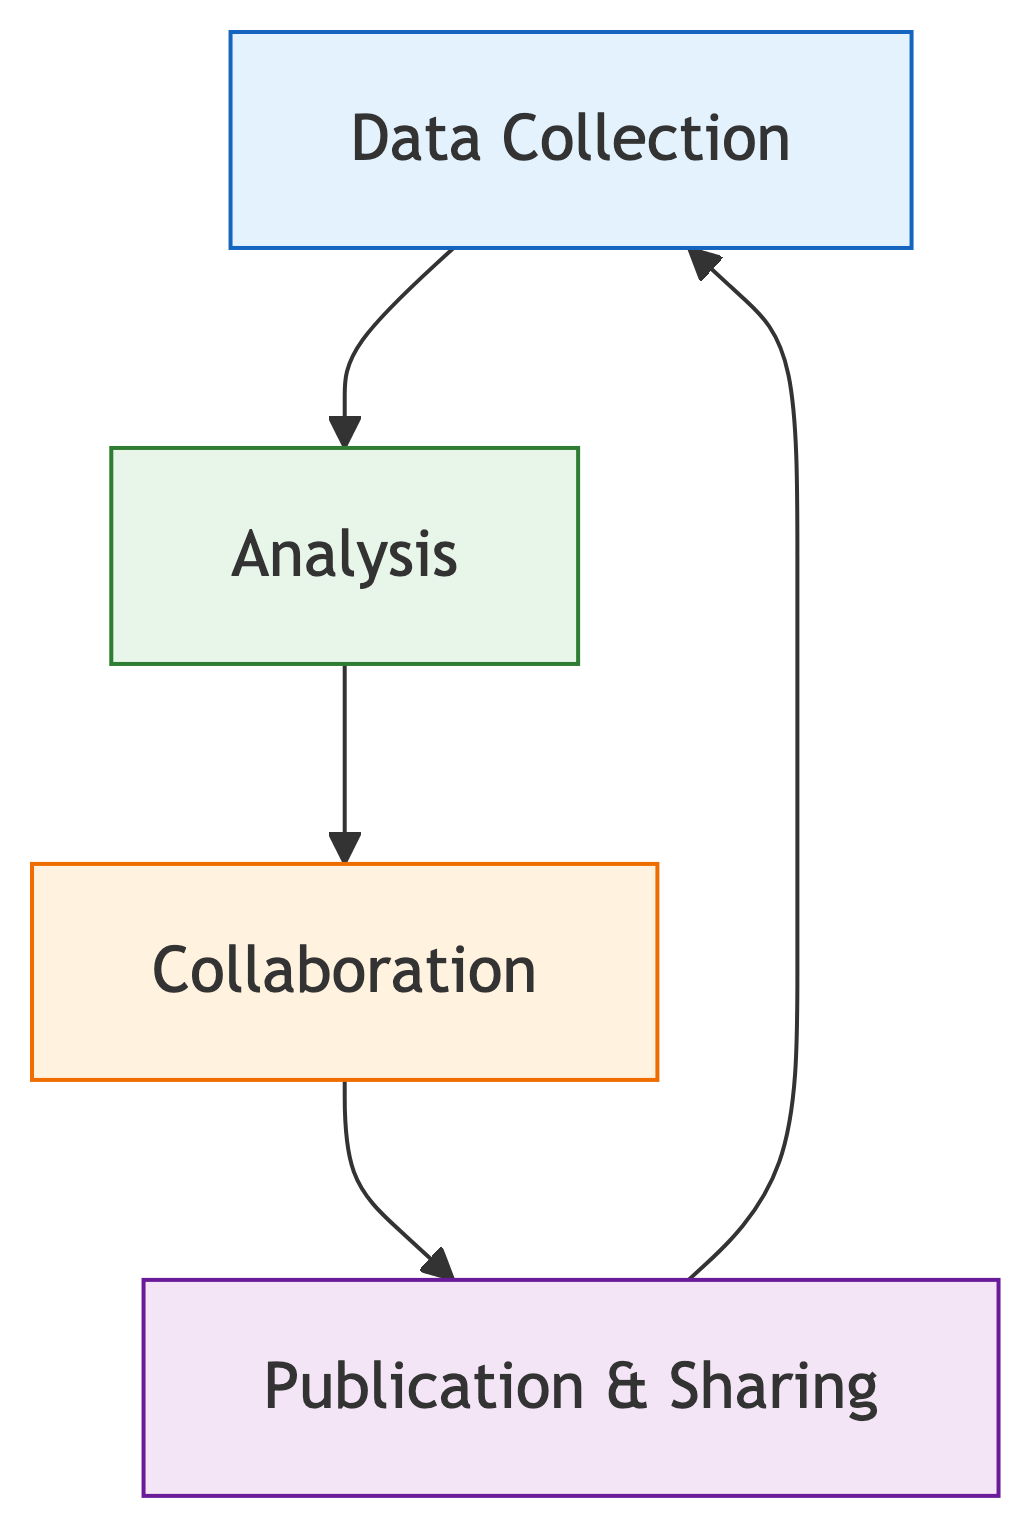
\includegraphics[width=2.68in,height=3.98in]{01-digital_tools_files/figure-latex/mermaid-figure-12.png}

\begin{quote}
🔁 \emph{Digital literacy underpins the entire cycle of modern
research.}
\end{quote}

\subsection{Addressing Common
Challenges}\label{addressing-common-challenges}

This course is about addressing the following challanges at a unversity
level.

\begin{longtable}[]{@{}
  >{\raggedright\arraybackslash}p{(\linewidth - 2\tabcolsep) * \real{0.3243}}
  >{\raggedright\arraybackslash}p{(\linewidth - 2\tabcolsep) * \real{0.6757}}@{}}
\toprule\noalign{}
\begin{minipage}[b]{\linewidth}\raggedright
Challenge
\end{minipage} & \begin{minipage}[b]{\linewidth}\raggedright
Digital Skills Response
\end{minipage} \\
\midrule\noalign{}
\endhead
\bottomrule\noalign{}
\endlastfoot
Disconnected research silos & Shared tools and workflows (Teams, GitHub,
RIS) \\
Data mismanagement & Version control, structured storage, FAIR
principles \\
Limited collaboration & Integrated communication and documentation
tools \\
Poor reproducibility & Use of open standards, coding literacy, and
transparent sharing \\
\end{longtable}

\begin{quote}
⚙️ \emph{Digital skills convert research challenges into structured
improvements.}
\end{quote}

\subsection{Collaboration Leads to Better
Research}\label{collaboration-leads-to-better-research}

Collaboration is at the heart of the DS\&DSP. By connecting researchers,
data professionals, and support specialists, the programme builds a
\textbf{community of digital practice} that strengthens the quality,
openness, and impact of research across disciplines.

\begin{quote}
``Collaboration is not an add-on---it is the mechanism through which
good research becomes great research.''
\end{quote}

\subsection{Programme Structure}\label{programme-structure}

The programme offers \textbf{three tiers of learning}, from foundational
to applied and specialist skills.

\begin{longtable}[]{@{}
  >{\raggedright\arraybackslash}p{(\linewidth - 4\tabcolsep) * \real{0.2667}}
  >{\raggedright\arraybackslash}p{(\linewidth - 4\tabcolsep) * \real{0.2667}}
  >{\raggedright\arraybackslash}p{(\linewidth - 4\tabcolsep) * \real{0.4667}}@{}}
\toprule\noalign{}
\begin{minipage}[b]{\linewidth}\raggedright
\textbf{Level}
\end{minipage} & \begin{minipage}[b]{\linewidth}\raggedright
\textbf{Focus}
\end{minipage} & \begin{minipage}[b]{\linewidth}\raggedright
\textbf{Example Modules}
\end{minipage} \\
\midrule\noalign{}
\endhead
\bottomrule\noalign{}
\endlastfoot
\textbf{Foundation} & Core digital research competencies & Essential
Digital Skills \\
\textbf{Intermediate} & Theory and collaboration in data science &
Python, R, Software Engineering \\
\textbf{Advanced} & Applied analysis and discipline-specific practice &
Bioinformatics, HPC, ML/AI \\
\end{longtable}

\begin{quote}
🧩 \emph{Each tier builds practical capability and supports research
independence.}
\end{quote}

\subsubsection{Courses}\label{courses}

\begin{longtable}[]{@{}
  >{\raggedright\arraybackslash}p{(\linewidth - 6\tabcolsep) * \real{0.2667}}
  >{\raggedright\arraybackslash}p{(\linewidth - 6\tabcolsep) * \real{0.5704}}
  >{\raggedright\arraybackslash}p{(\linewidth - 6\tabcolsep) * \real{0.1185}}
  >{\raggedright\arraybackslash}p{(\linewidth - 6\tabcolsep) * \real{0.0444}}@{}}
\toprule\noalign{}
\begin{minipage}[b]{\linewidth}\raggedright
Course
\end{minipage} & \begin{minipage}[b]{\linewidth}\raggedright
Description
\end{minipage} & \begin{minipage}[b]{\linewidth}\raggedright
Duration
\end{minipage} & \begin{minipage}[b]{\linewidth}\raggedright
Note
\end{minipage} \\
\midrule\noalign{}
\endhead
\bottomrule\noalign{}
\endlastfoot
Essential Digital Skills -- Foundation & Introduces the tools,
practices, and principles needed to participate confidently in digital
research. & 4× half days & \\
Methods for Data Science -- Theoretical & Introduces coding, software,
and collaboration practices needed for sustainable research. & 4× half
days & \\
Methods for Data Science -- Applied Python & Provides practical
experience in data analysis and interpretation using Python. & 2 days &
Introductory and intermediate \\
Methods for Data Science -- Applied R & Provides practical experience in
data analysis and interpretation using R. & 2 days & Introductory and
intermediate \\
Advanced & --- & 1 day? & AI? ML? Bioinformatics? \\
\end{longtable}

\begin{center}\rule{0.5\linewidth}{0.5pt}\end{center}

\paragraph{Task 1: Digital Skills
Reflection}\label{task-1-digital-skills-reflection}

Let's start by reflecting on your current digital research skills.

❓ \emph{What's digital skills or tool you want to develop this year?}

\phantomsection\label{frame-q1}

\section{Institutional Systems for Digital
Research}\label{institutional-systems-for-digital-research}

\begin{center}
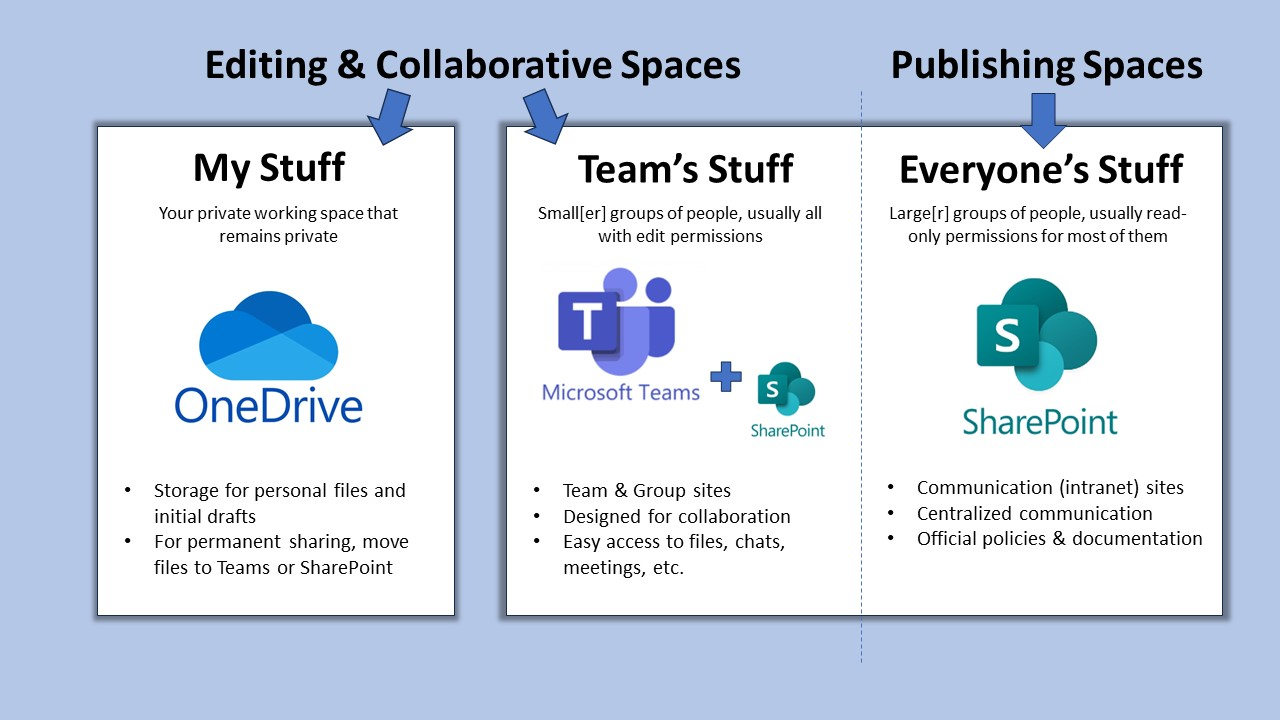
\includegraphics[width=5.20833in,height=\textheight,keepaspectratio]{fig/sharepoint.png}
\end{center}

\subsection{Why Institutional Systems
Matter}\label{why-institutional-systems-matter}

Digital research depends on \textbf{connected systems} that enable
collaboration, safeguard data, and streamline research workflows.

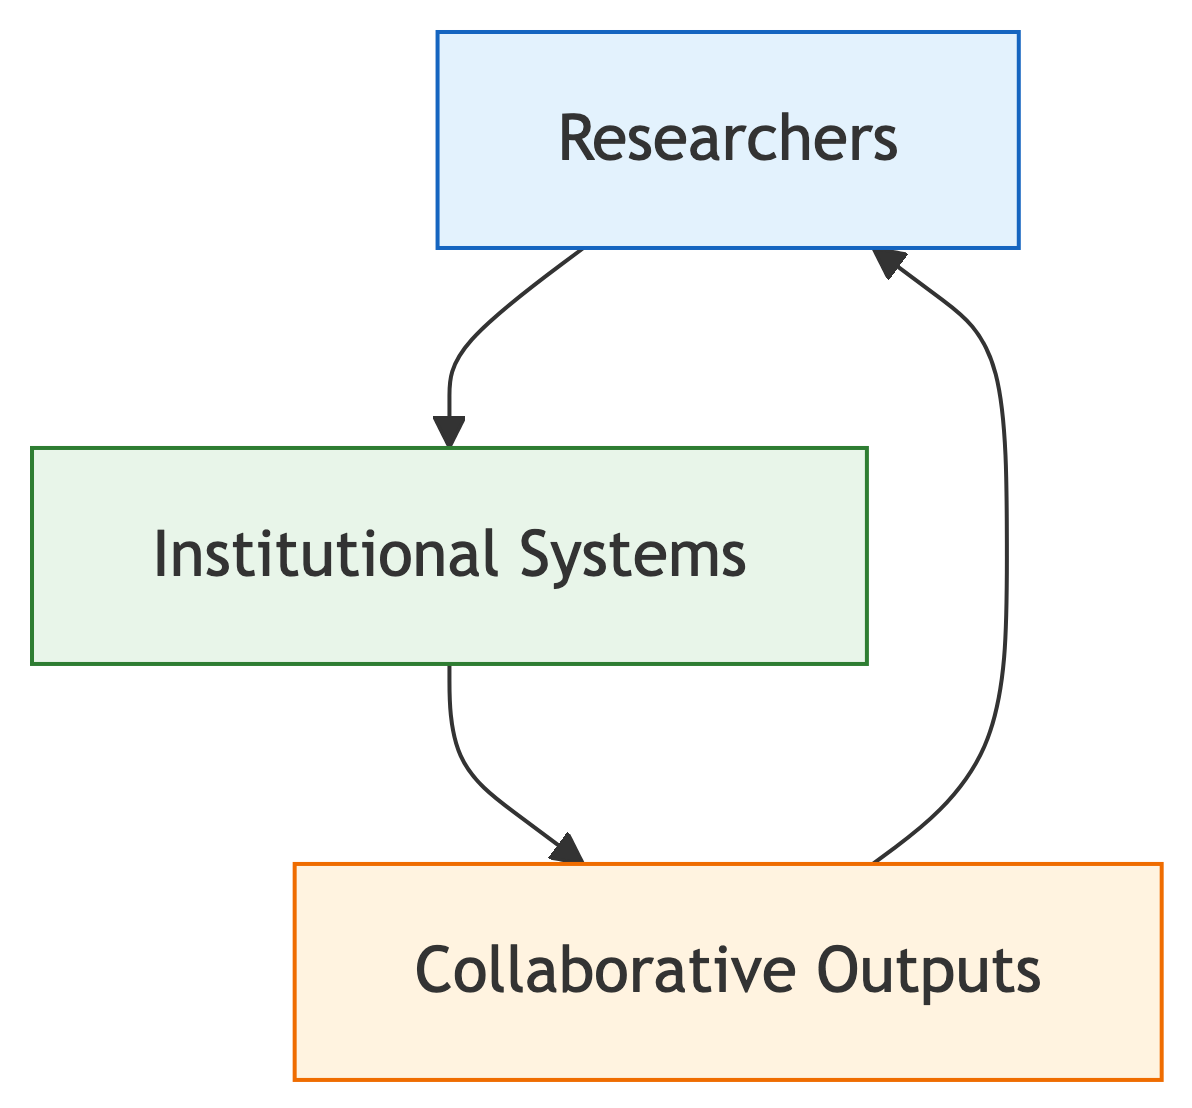
\includegraphics[width=3.11in,height=2.9in]{01-digital_tools_files/figure-latex/mermaid-figure-11.png}

\begin{quote}
🧩 \emph{Institutional systems form the backbone of a connected research
ecosystem.}
\end{quote}

\subsection{UoN's Digital Ecosystem}\label{uons-digital-ecosystem}

At the University of Nottingham, research operates within a
\textbf{digitally integrated environment} that connects people, data,
and administration.

\begin{longtable}[]{@{}ll@{}}
\toprule\noalign{}
\textbf{System} & \textbf{Primary Role} \\
\midrule\noalign{}
\endhead
\bottomrule\noalign{}
\endlastfoot
\textbf{Microsoft 365} & Collaboration and communication \\
\textbf{SharePoint} & Long-term data and document sharing \\
\textbf{UniCore} & Finance, HR, and procurement \\
\textbf{RIS (Worktribe)} & Research lifecycle, funding, outputs \\
\end{longtable}

\begin{quote}
🏛️ \emph{Together these platforms enable secure, collaborative, and
transparent research practice.}
\end{quote}

\subsection{Microsoft 365: A Platform for
Collaboration}\label{microsoft-365-a-platform-for-collaboration}

Microsoft 365 supports daily research activity---from communication to
data management---within a single, integrated workspace.

\begin{longtable}[]{@{}ll@{}}
\toprule\noalign{}
\textbf{Tool} & \textbf{Function} \\
\midrule\noalign{}
\endhead
\bottomrule\noalign{}
\endlastfoot
\textbf{Word \& Excel} & Writing, data capture, and co-editing \\
\textbf{OneDrive} & Personal cloud storage with versioning \\
\textbf{Teams} & Communication, meetings, shared workspaces \\
\textbf{SharePoint} & Institutional document repositories \\
\end{longtable}

\begin{quote}
💬 \emph{Microsoft 365 is the shared workspace for modern research
collaboration.}
\end{quote}

\subsection{Collaboration in Practice}\label{collaboration-in-practice}

Microsoft 365 enables seamless teamwork across roles and locations.

\begin{itemize}
\tightlist
\item
  Co-edit documents with real-time version tracking\\
\item
  Use Teams for context-based discussion and meetings\\
\item
  Store project materials in structured SharePoint libraries\\
\item
  Sync files through OneDrive for offline access
\end{itemize}

\begin{quote}
🔁 \emph{Integrated tools make collaborative research smooth, secure,
and efficient.}
\end{quote}

\subsection{File Collaboration Best
Practice}\label{file-collaboration-best-practice}

\begin{itemize}
\tightlist
\item
  Use \textbf{Teams or SharePoint} for shared project files\\
\item
  Enable \textbf{autosave and version history} in Word or Excel\\
\item
  Maintain \textbf{logical folder structures} by project phase\\
\item
  Apply \textbf{permissions and access control} with care
\end{itemize}

\begin{quote}
🧠 \emph{Good file management is the foundation of digital
reproducibility.}
\end{quote}

\subsection{UniCore and RIS: Institutional
Systems}\label{unicore-and-ris-institutional-systems}

UniCore and RIS link the operational and administrative sides of
research.

\begin{longtable}[]{@{}
  >{\raggedright\arraybackslash}p{(\linewidth - 2\tabcolsep) * \real{0.5000}}
  >{\raggedright\arraybackslash}p{(\linewidth - 2\tabcolsep) * \real{0.5000}}@{}}
\toprule\noalign{}
\begin{minipage}[b]{\linewidth}\raggedright
\textbf{System}
\end{minipage} & \begin{minipage}[b]{\linewidth}\raggedright
\textbf{Purpose}
\end{minipage} \\
\midrule\noalign{}
\endhead
\bottomrule\noalign{}
\endlastfoot
\textbf{UniCore} & Finance, HR, procurement, and resource management \\
\textbf{RIS (Worktribe)} & Project proposals, outputs, and compliance
tracking \\
\end{longtable}

\begin{quote}
🗂️ \emph{These systems ensure research activity is visible, auditable,
and supported.}
\end{quote}

\subsection{UniCore Overview}\label{unicore-overview}

\textbf{UniCore} is UoN's enterprise system for managing finance, HR,
and procurement.

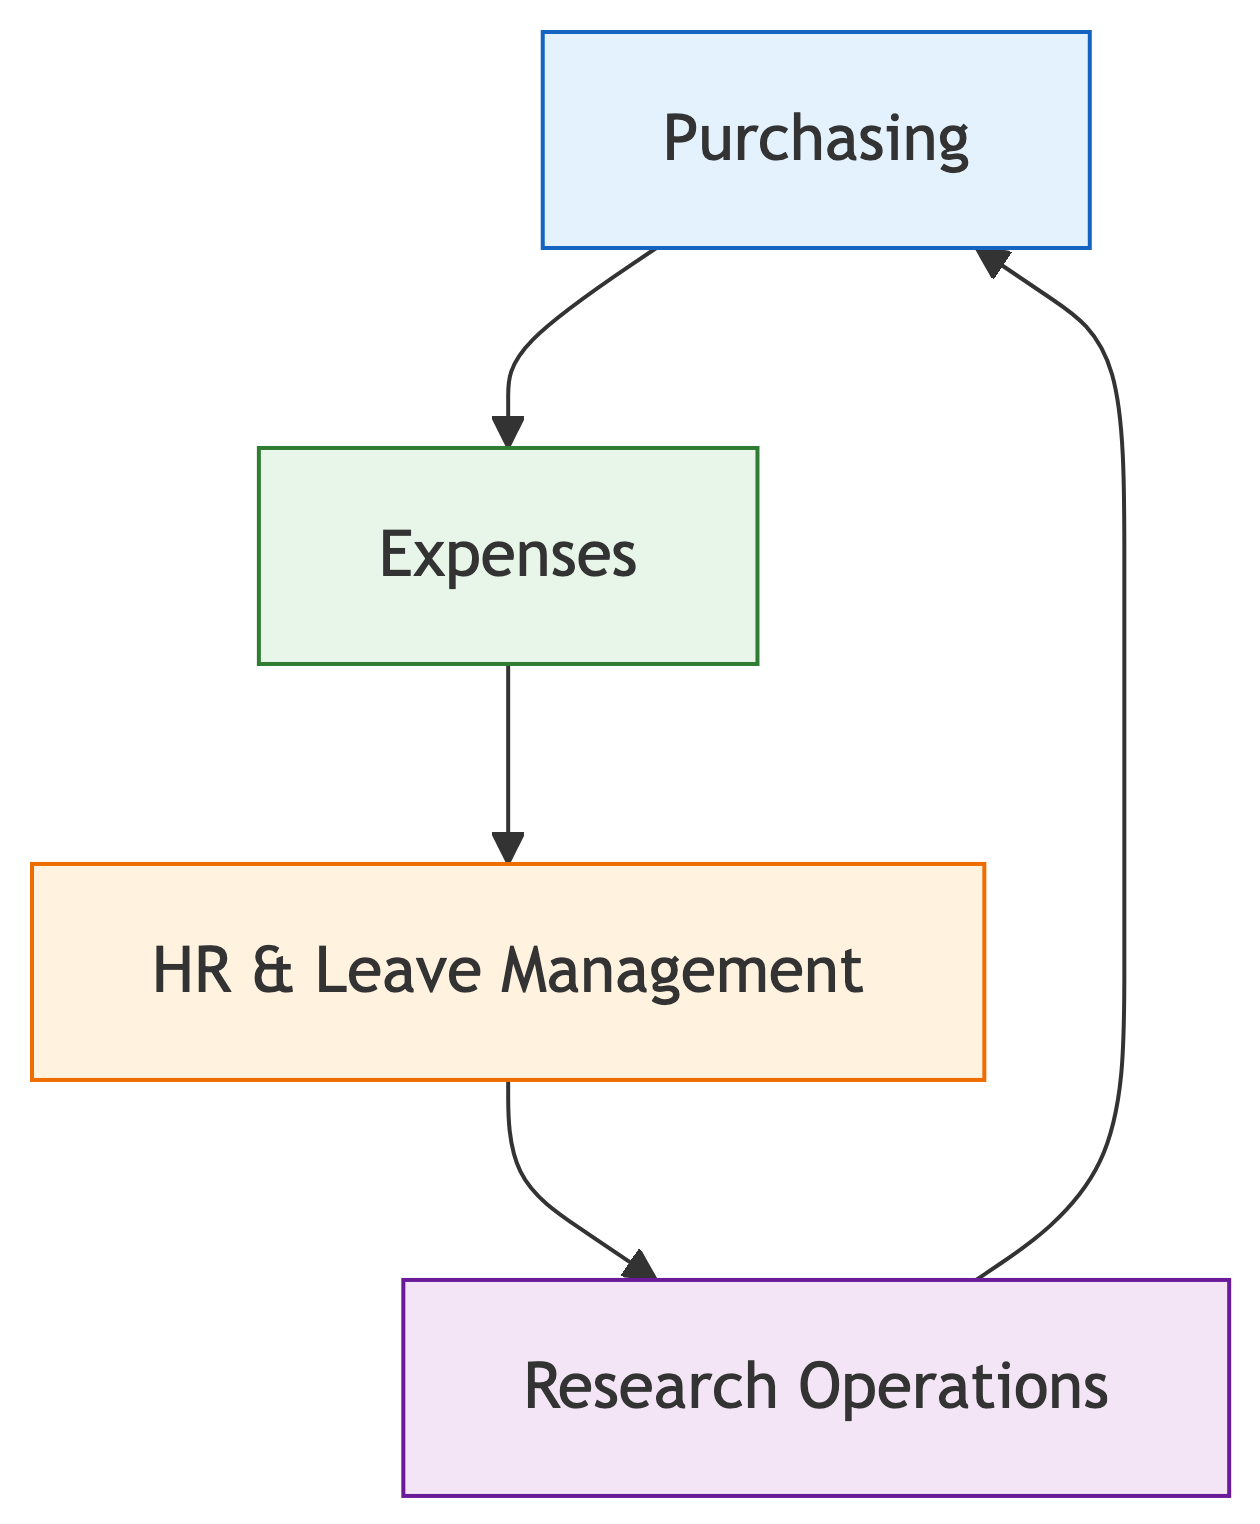
\includegraphics[width=3.28in,height=3.98in]{01-digital_tools_files/figure-latex/mermaid-figure-10.png}

\begin{quote}
🧭 \emph{UniCore underpins the financial and operational side of
research.}
\end{quote}

\subsection{RIS (Research Information
System)}\label{ris-research-information-system}

\textbf{RIS (Worktribe)} records, tracks, and reports the full research
lifecycle.

\begin{longtable}[]{@{}ll@{}}
\toprule\noalign{}
\textbf{Feature} & \textbf{Purpose} \\
\midrule\noalign{}
\endhead
\bottomrule\noalign{}
\endlastfoot
\textbf{Grant Management} & Develop and cost funding proposals \\
\textbf{Outputs Tracking} & Record publications and datasets \\
\textbf{Impact Recording} & Capture engagement and REF evidence \\
\textbf{ORCID Integration} & Synchronise researcher identity and
outputs \\
\end{longtable}

\begin{quote}
📚 \emph{RIS ensures research activity is captured and connected
institutionally.}
\end{quote}

\subsection{Integrated Research
Systems}\label{integrated-research-systems}

The strength of UoN's infrastructure lies in \textbf{interoperability}
--- connecting research activity, collaboration, and administration.

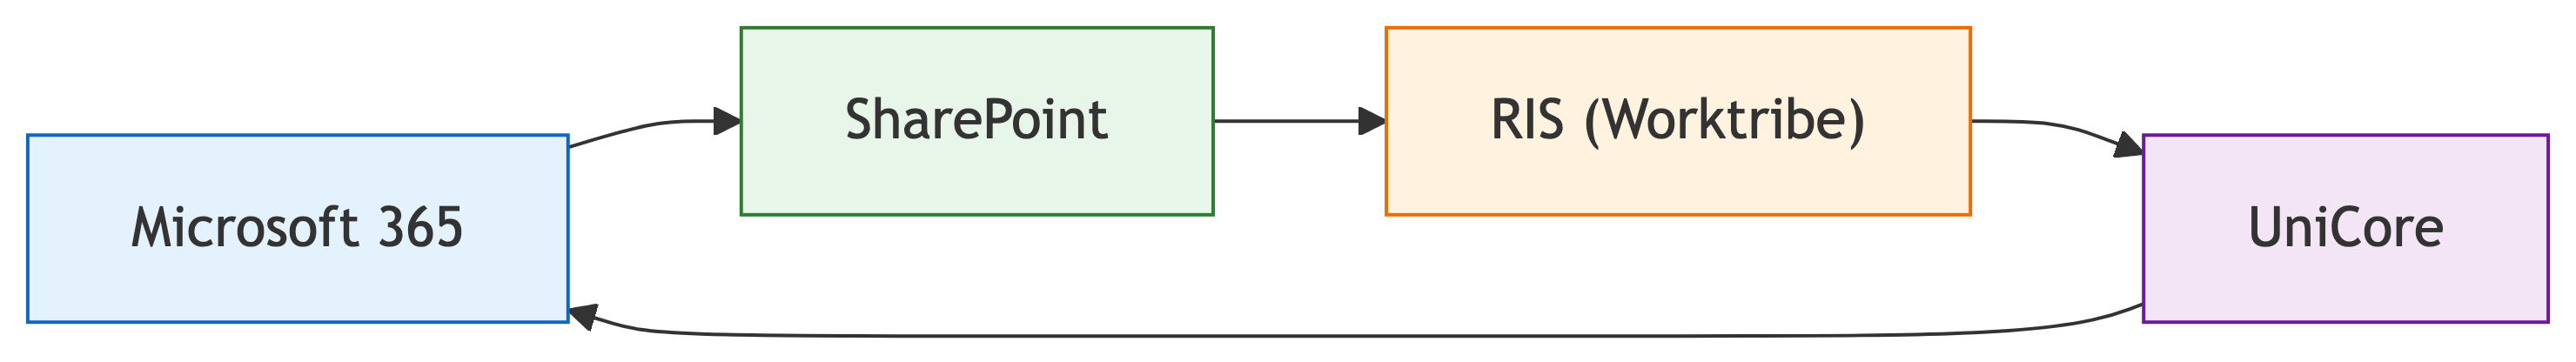
\includegraphics[width=7.74in,height=1.09in]{01-digital_tools_files/figure-latex/mermaid-figure-9.png}

\begin{quote}
🔗 \emph{Connectivity between systems ensures seamless movement from
idea to output.}
\end{quote}

\subsection{System Use in Context}\label{system-use-in-context}

\begin{longtable}[]{@{}
  >{\raggedright\arraybackslash}p{(\linewidth - 4\tabcolsep) * \real{0.2778}}
  >{\raggedright\arraybackslash}p{(\linewidth - 4\tabcolsep) * \real{0.3333}}
  >{\raggedright\arraybackslash}p{(\linewidth - 4\tabcolsep) * \real{0.3889}}@{}}
\toprule\noalign{}
\begin{minipage}[b]{\linewidth}\raggedright
\textbf{Research Task}
\end{minipage} & \begin{minipage}[b]{\linewidth}\raggedright
\textbf{Recommended System}
\end{minipage} & \begin{minipage}[b]{\linewidth}\raggedright
\textbf{Collaboration Benefit}
\end{minipage} \\
\midrule\noalign{}
\endhead
\bottomrule\noalign{}
\endlastfoot
Co-author a paper & OneDrive / Word & Real-time editing and version
control \\
Submit a funding bid & RIS & Shared proposal development and audit
trail \\
Claim expenses & UniCore & Secure and traceable reimbursement \\
Share datasets & SharePoint / Teams & Controlled access and
persistence \\
Record outputs & RIS + ORCID & Automatic institutional linking \\
\end{longtable}

\begin{quote}
⚙️ \emph{Each platform serves a distinct role in the research
ecosystem.}
\end{quote}

\subsection{The Broader Vision: Connected
Research}\label{the-broader-vision-connected-research}

By using institutional systems effectively teams build \textbf{trust and
accountability}, data remains \textbf{secure, reusable, and open} and
researchers can spend more time working on \textbf{innovation and
discovery}

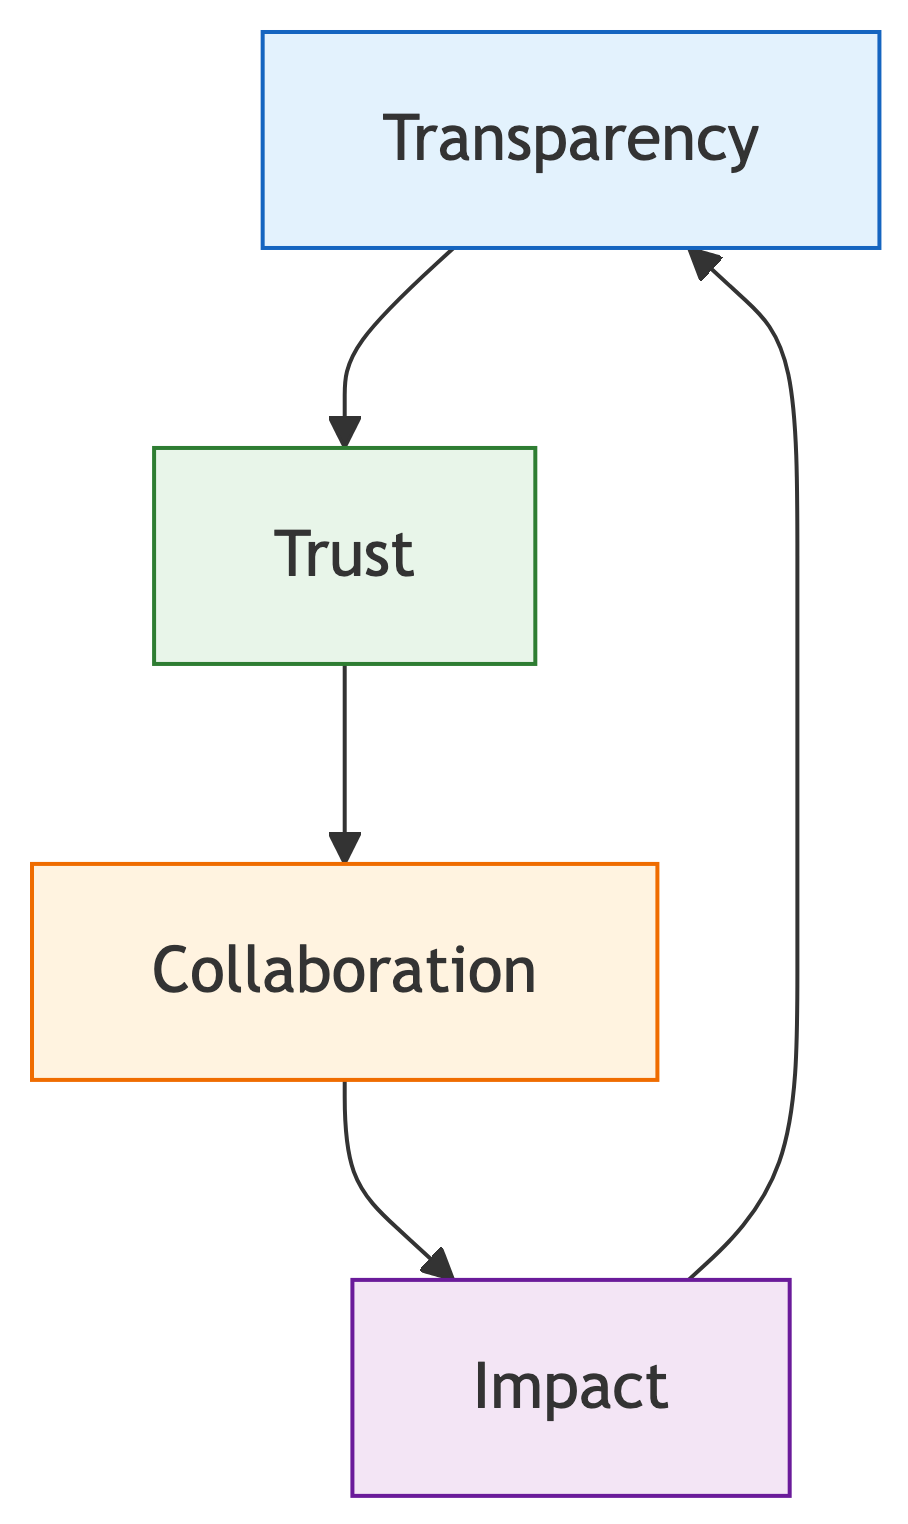
\includegraphics[width=2.37in,height=3.98in]{01-digital_tools_files/figure-latex/mermaid-figure-8.png}

\begin{quote}
🌍 \emph{Digital infrastructure is the connective tissue of modern
research.}
\end{quote}

\begin{center}\rule{0.5\linewidth}{0.5pt}\end{center}

\paragraph{Task 2: Match Research Tasks to
Tools}\label{task-2-match-research-tasks-to-tools}

\paragraph{Activity}

In groups of 4-5, discuss and list the digital tools you would use for
each of the following:

\begin{enumerate}
\def\labelenumi{\arabic{enumi}.}
\tightlist
\item
  Co-write a manuscript\\
\item
  Submit a funding bid\\
\item
  Order equipment\\
\item
  Share large datasets with your team
\end{enumerate}

\paragraph{Cohort Answers}

\phantomsection\label{frame-q2}

\paragraph{Reflection}

\begin{itemize}
\tightlist
\item
  Share your answers with the plenary\\
\item
  Reflect on whether you've used any of these systems before\\
\item
  Identify any gaps in your familiarity that you want to address
\end{itemize}

\paragraph{Answers}

\begin{itemize}
\tightlist
\item
  \textbf{Microsoft Word -\textgreater{} Sharepoint + Teams} are ideal
  for collaborative document editing\\
\item
  \textbf{RIS (Worktribe)} is used for grant applications and research
  output tracking\\
\item
  \textbf{UniCore} handles finance, procurement, HR and expenses\\
\item
  \textbf{Microsoft Teams + SharePoint} is best for long-term group file
  access and collaboration\\
\end{itemize}

\section{Research Identity \&
Profiles}\label{research-identity-profiles}

\begin{center}

\includegraphics[width=5.20833in,height=\textheight,keepaspectratio]{fig/orchid.png}
\end{center}

\subsection{Why Research Identity
Matters}\label{why-research-identity-matters}

Your \textbf{research identity} defines how your work is discovered,
attributed, and connected across the digital research ecosystem.

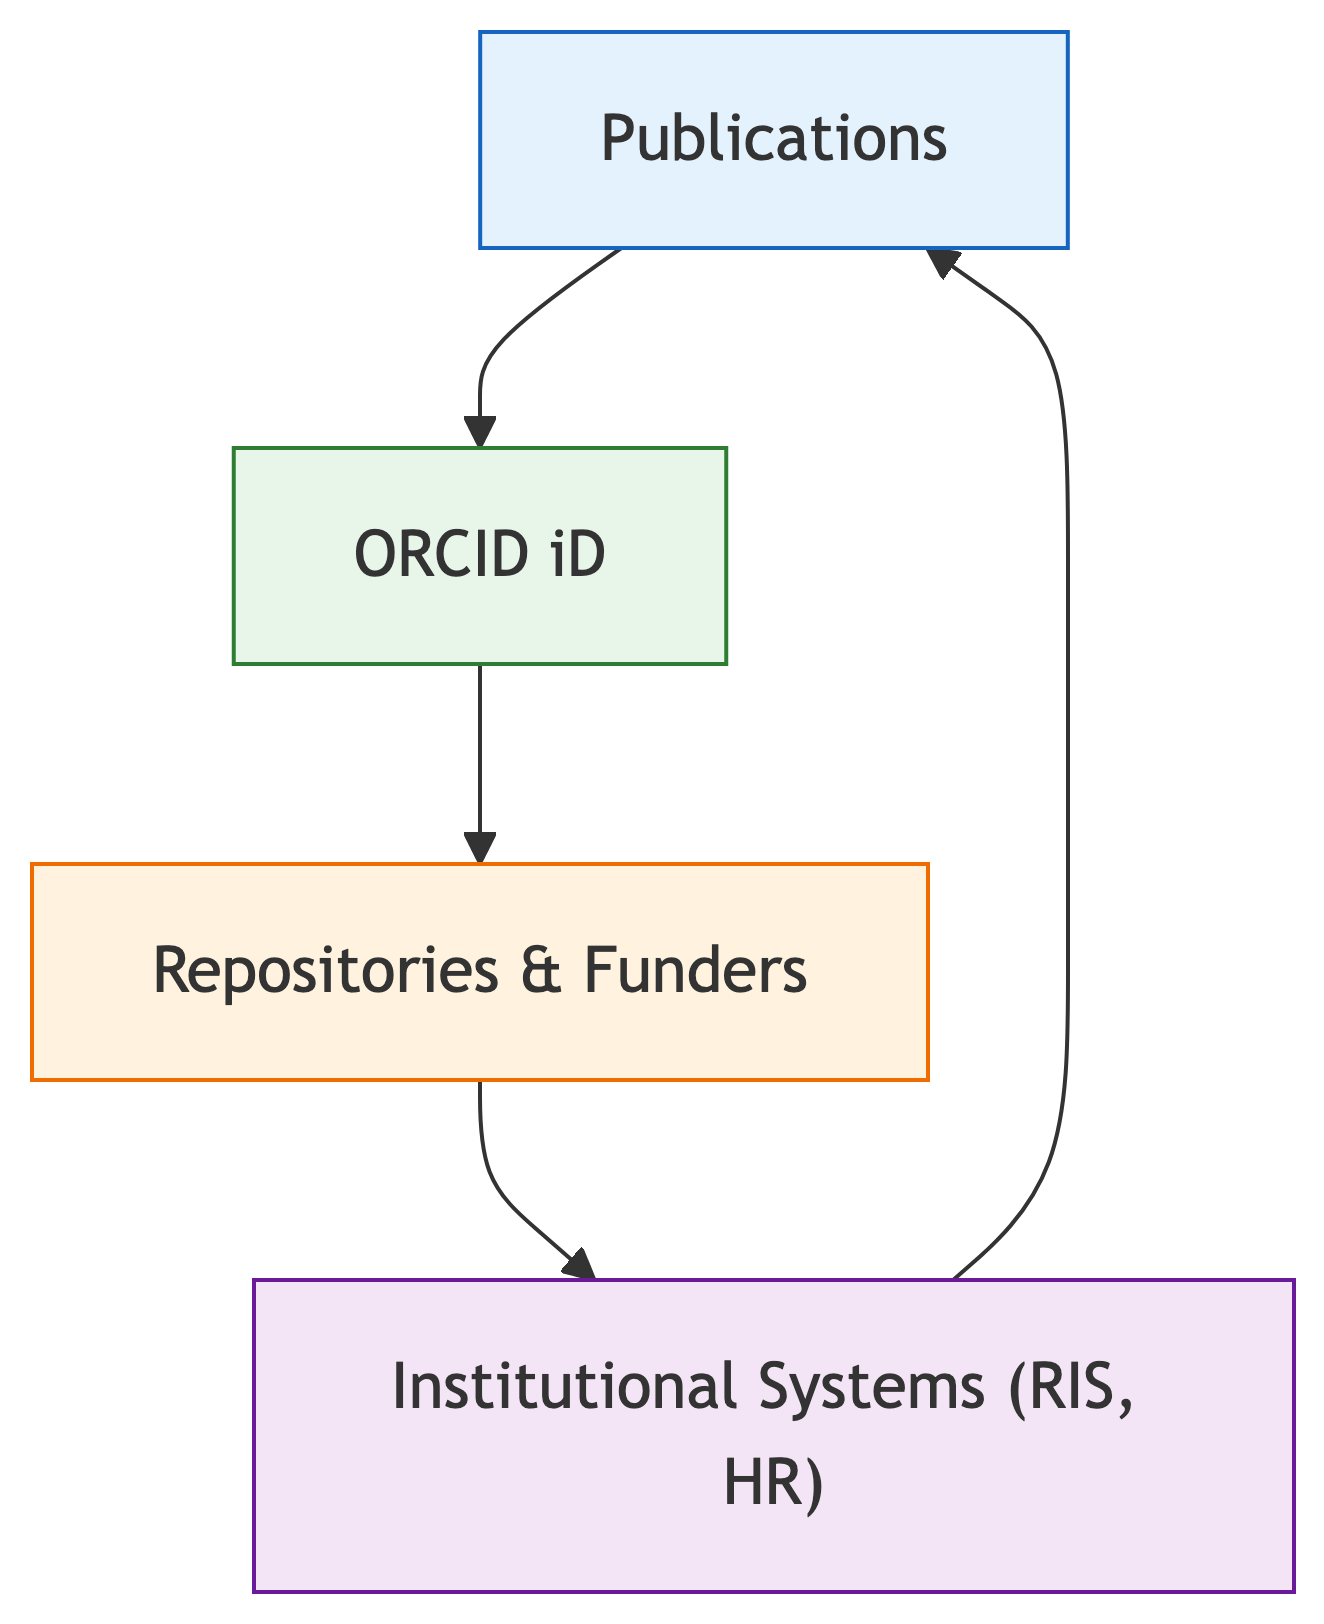
\includegraphics[width=3.45in,height=4.23in]{01-digital_tools_files/figure-latex/mermaid-figure-7.png}

\begin{quote}
🧩 \emph{A coherent digital identity ensures your contributions are
visible, citable, and connected.}
\end{quote}

\subsection{The Importance of
Consistency}\label{the-importance-of-consistency}

A consistent identity links your outputs, affiliations, and roles
automatically across systems.\\
This guarantees proper attribution and supports efficient collaboration.

\begin{itemize}
\tightlist
\item
  Ensures \textbf{discoverability} across publishers and repositories\\
\item
  Prevents \textbf{duplication or misattribution} of outputs\\
\item
  Facilitates \textbf{integration} with institutional systems like RIS
\end{itemize}

\begin{quote}
💡 \emph{A consistent research identity builds long-term recognition and
credibility.}
\end{quote}

\subsection{ORCID: A Persistent Digital
Identifier}\label{orcid-a-persistent-digital-identifier}

\textbf{ORCID (Open Researcher and Contributor ID)} is the global
standard for uniquely identifying researchers across institutions and
disciplines.

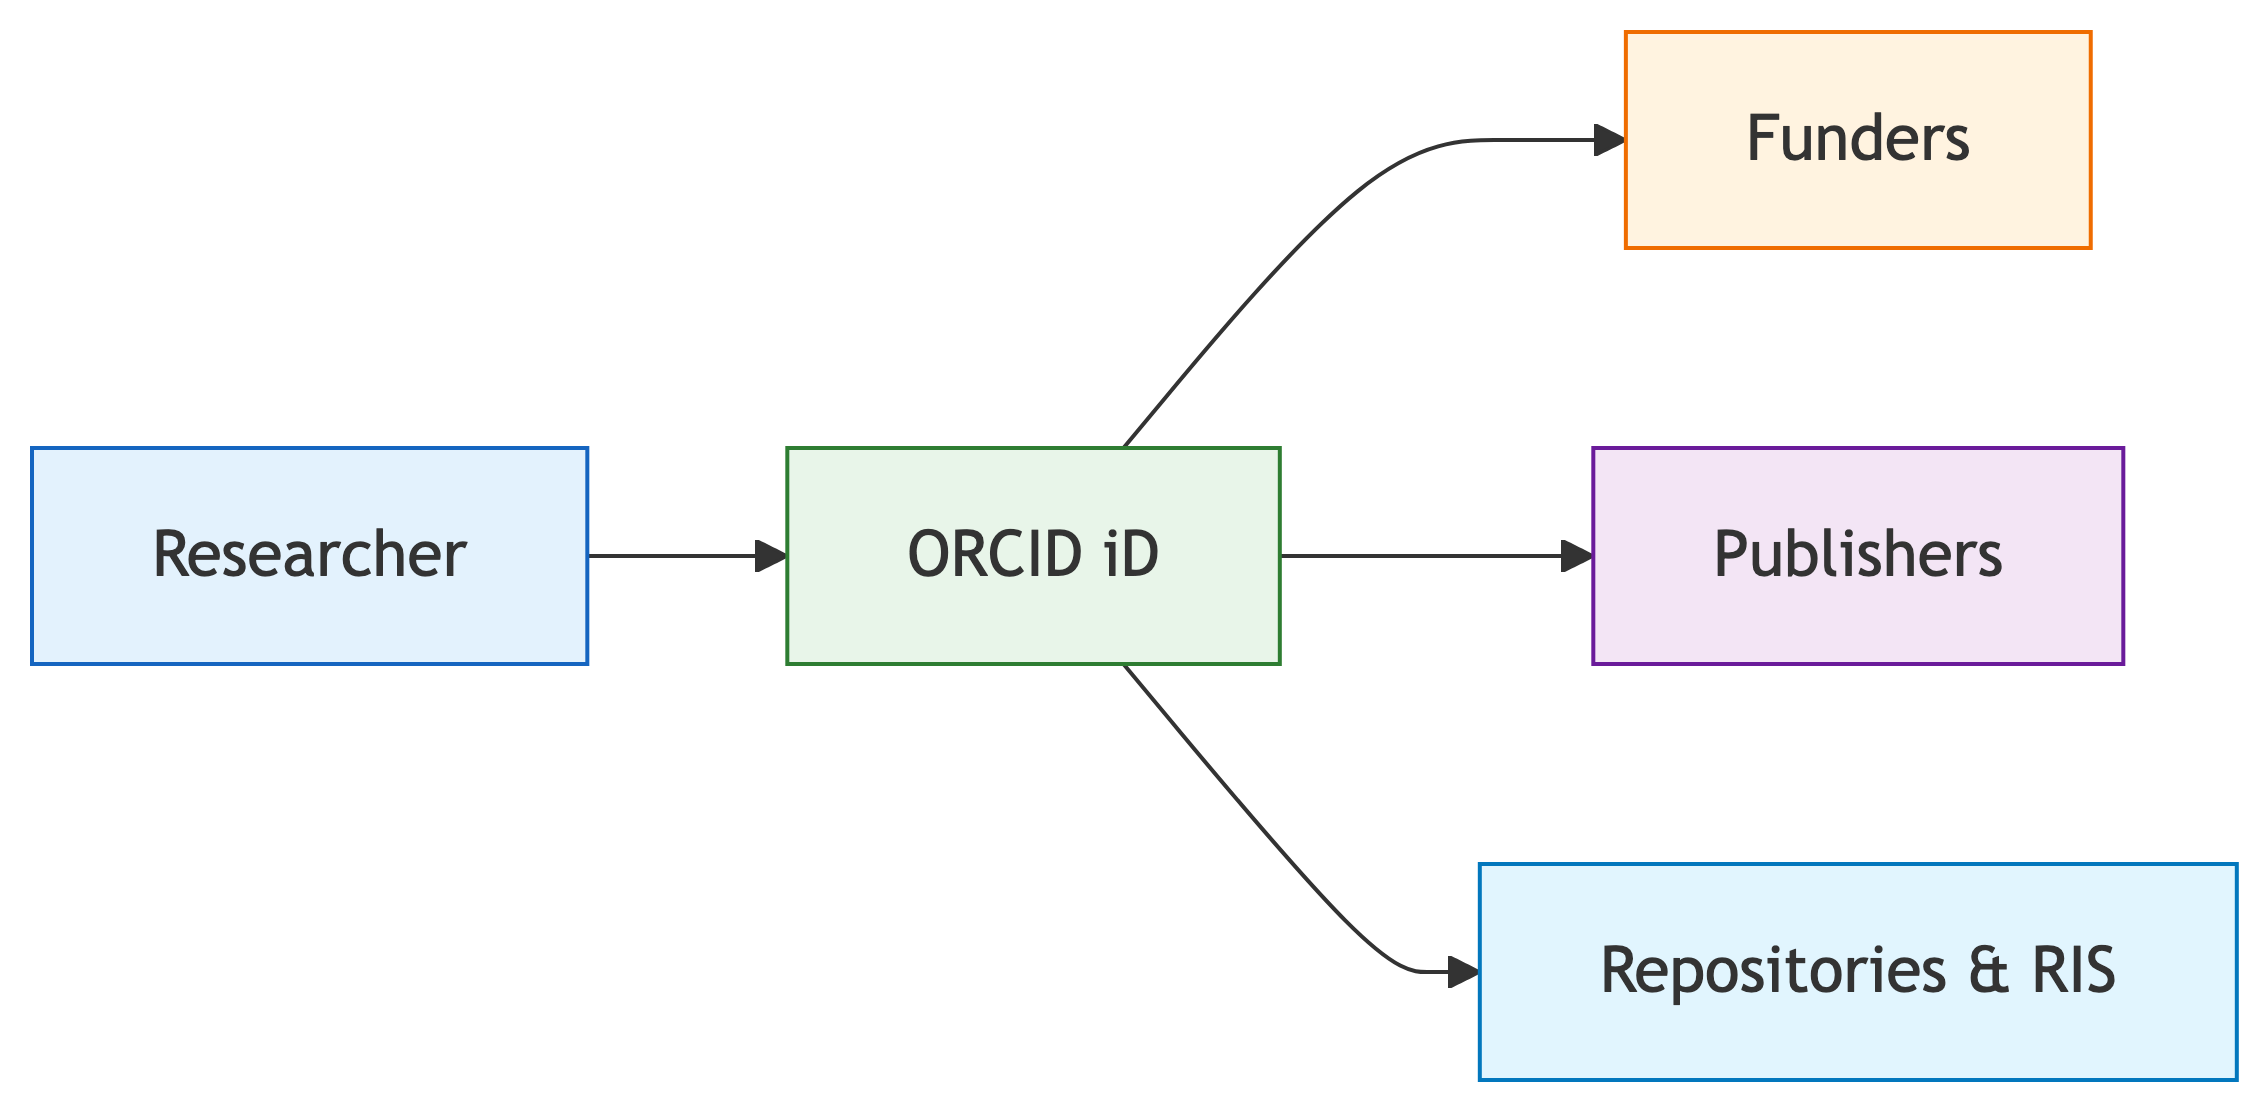
\includegraphics[width=5.91in,height=2.9in]{01-digital_tools_files/figure-latex/mermaid-figure-6.png}

\begin{quote}
🧠 \emph{Your ORCID iD is your digital fingerprint across the global
research ecosystem.}
\end{quote}

\subsection{Why ORCID is Essential}\label{why-orcid-is-essential}

\begin{itemize}
\tightlist
\item
  \textbf{Universal interoperability:} used by funders, publishers, and
  institutions\\
\item
  \textbf{Automatic updates:} Crossref and DataCite can sync new
  outputs\\
\item
  \textbf{Portability:} your iD remains active throughout your career
\end{itemize}

\begin{quote}
🔗 \emph{ORCID connects your research identity beyond institutional
boundaries.}
\end{quote}

\subsection{RIS (Research Information System) at
UoN}\label{ris-research-information-system-at-uon}

At UoN, \textbf{RIS (Worktribe)} complements your ORCID profile by
linking research activity to institutional records.

\begin{longtable}[]{@{}ll@{}}
\toprule\noalign{}
\textbf{Feature} & \textbf{Function} \\
\midrule\noalign{}
\endhead
\bottomrule\noalign{}
\endlastfoot
\textbf{Grant Management} & Tracks proposals, approvals, and costings \\
\textbf{Outputs Dashboard} & Records publications, datasets, and
impacts \\
\textbf{Compliance} & Supports REF and Open Access requirements \\
\textbf{Integration} & Syncs with ORCID and external repositories \\
\end{longtable}

\begin{quote}
🏛️ \emph{RIS ensures your institutional identity mirrors your global
research presence.}
\end{quote}

\subsection{ORCID--RIS Integration}\label{orcidris-integration}

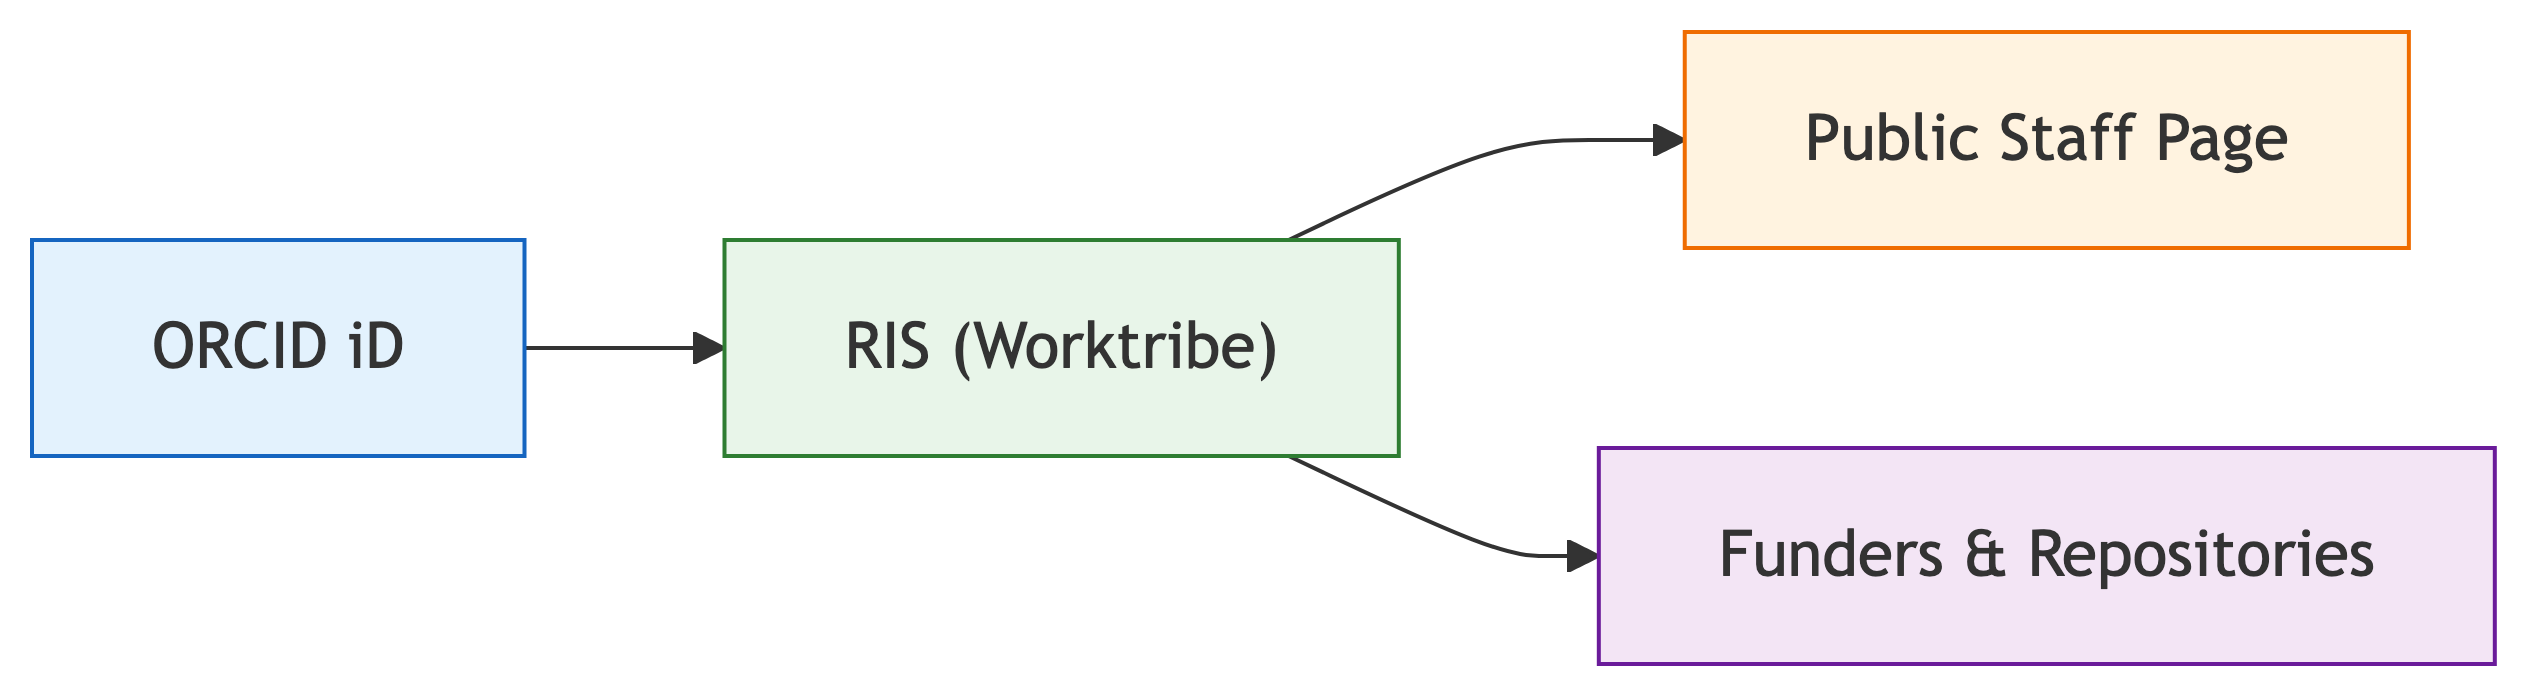
\includegraphics[width=6.58in,height=1.81in]{01-digital_tools_files/figure-latex/mermaid-figure-5.png}

\begin{quote}
💬 \emph{Connecting ORCID to RIS automates data flow and strengthens
institutional visibility.}
\end{quote}

\subsection{Scholarly Profiles Across
Systems}\label{scholarly-profiles-across-systems}

Different platforms amplify your professional presence.\\
When synchronised with ORCID, they create a distributed network of your
scholarly identity.

\begin{longtable}[]{@{}
  >{\raggedright\arraybackslash}p{(\linewidth - 4\tabcolsep) * \real{0.3846}}
  >{\raggedright\arraybackslash}p{(\linewidth - 4\tabcolsep) * \real{0.3333}}
  >{\raggedright\arraybackslash}p{(\linewidth - 4\tabcolsep) * \real{0.2821}}@{}}
\toprule\noalign{}
\begin{minipage}[b]{\linewidth}\raggedright
\textbf{Platform}
\end{minipage} & \begin{minipage}[b]{\linewidth}\raggedright
\textbf{Purpose}
\end{minipage} & \begin{minipage}[b]{\linewidth}\raggedright
\textbf{Notes}
\end{minipage} \\
\midrule\noalign{}
\endhead
\bottomrule\noalign{}
\endlastfoot
\textbf{Scopus Author ID} & Tracks citations, co-authorship, and
affiliations & Merge duplicates for accuracy \\
\textbf{Google Scholar} & Monitors visibility and citation trends &
Manual curation may be required \\
\textbf{ResearchGate / Academia.edu} & Social exchange platforms & Use
responsibly; metrics are non-standard \\
\end{longtable}

\begin{quote}
⚠️ \emph{Prioritise verified systems like ORCID, Scopus, and RIS for
credible visibility.}
\end{quote}

\subsection{Managing Your Research
Profiles}\label{managing-your-research-profiles}

\begin{itemize}
\tightlist
\item
  Make your \textbf{ORCID profile public} for discoverability\\
\item
  \textbf{Merge duplicate Scopus IDs} to ensure accuracy\\
\item
  \textbf{Link ORCID to RIS} for automatic synchronisation\\
\item
  Use consistent \textbf{name and affiliation formats}\\
\item
  Avoid unverified or \textbf{proprietary metrics}\\
\item
  \textbf{Audit profiles regularly} for correctness
\end{itemize}

\begin{quote}
🧭 \emph{Managing your identity actively ensures your research remains
visible and verifiable.}
\end{quote}

\subsection{Research Identity as Collaboration
Infrastructure}\label{research-identity-as-collaboration-infrastructure}

A connected identity supports collaboration, attribution, and trust
across teams.


\includegraphics[width=3.39in,height=3.98in]{01-digital_tools_files/figure-latex/mermaid-figure-4.png}

\begin{quote}
🤝 \emph{A well-managed identity connects people, data, and recognition
across research networks.}
\end{quote}

\subsection{The Broader Impact of a Connected
Identity}\label{the-broader-impact-of-a-connected-identity}

\begin{itemize}
\tightlist
\item
  Enhances \textbf{interdisciplinary visibility}\\
\item
  Simplifies \textbf{authorship and data attribution}\\
\item
  Strengthens \textbf{institutional reporting} and compliance\\
\item
  Promotes \textbf{open, transparent research collaboration}
\end{itemize}

\begin{quote}
🌍 \emph{A connected identity enables connected research.}
\end{quote}

\begin{center}\rule{0.5\linewidth}{0.5pt}\end{center}

\paragraph{Task 3: Research Identity
Self-Audit}\label{task-3-research-identity-self-audit}

\paragraph{Activity part 1}

❓ Do you have a ORCID research identity?

Visit \href{https://orcid.org/}{Orcid}, Log in / sign up

\paragraph{Activity part 2}

❓ Is your ORCID iD is populated with your name, affiliation etc? if not
make sure that is complete. - Set your ORCID ID to public (if
appropriate)

\paragraph{Further Infomation}

\begin{itemize}
\tightlist
\item
  You can actually link your RIS and ORCID profiles but for that you
  need to be registered to use worktribe. It is recomended that you
  \href{https://nottingham-research.worktribe.com/login.jx}{request
  access}
\item
  Once registered and logged in, you can link your ORCID and RIS
  profiles. For more infomation please refer to the
  \href{http://moodle.nottingham.ac.uk/course/view.php?id=47898}{RIS
  training materials} to go away and read
\end{itemize}

\section{Digital Security \& Good
Practice}\label{digital-security-good-practice}

\begin{center}
\includegraphics[width=5.20833in,height=\textheight,keepaspectratio]{fig/security.png}
\end{center}

\subsection{Why Digital Security
Matters}\label{why-digital-security-matters}

Effective digital research requires vigilance, responsibility, and sound
data stewardship.\\
Security protects not only your research, but also your collaborators
and institution.


\includegraphics[width=2.86in,height=5.06in]{01-digital_tools_files/figure-latex/mermaid-figure-3.png}

\begin{quote}
🔒 \emph{Digital security is a collective responsibility---protecting
data protects discovery.}
\end{quote}

\subsection{Passwords \& Access
Management}\label{passwords-access-management}

Passwords remain the first line of defence against unauthorised
access.\\
Weak or reused passwords are still the most common research
vulnerability.

\begin{itemize}
\tightlist
\item
  Use \textbf{at least 12 characters} with a mix of cases, numbers, and
  symbols\\
\item
  Create \textbf{unique passwords} for each system\\
\item
  Never share credentials via email or chat\\
\item
  Regularly \textbf{review access permissions} for shared platforms
\end{itemize}

\begin{quote}
🧠 \emph{Strong passwords are simple, low-cost defences against complex
risks.}
\end{quote}

\subsection{Multi-Factor Authentication
(MFA)}\label{multi-factor-authentication-mfa}

\textbf{MFA} adds a crucial verification step beyond a password.\\
Even if your password is compromised, MFA prevents most unauthorised
logins.

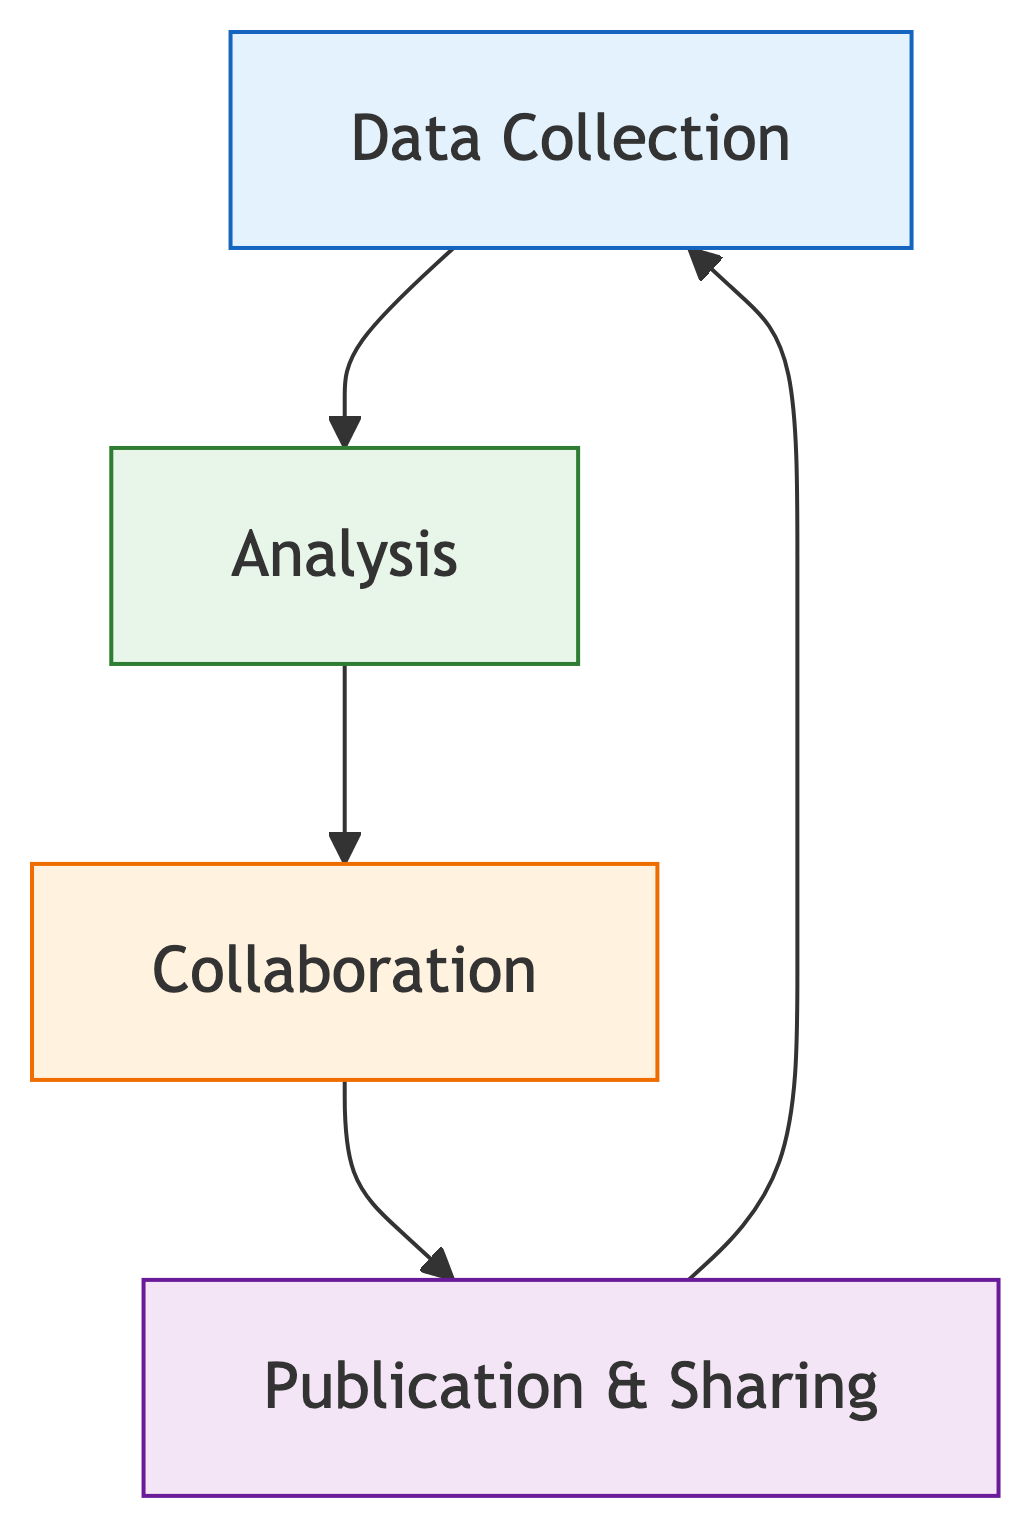
\includegraphics[width=8.91in,height=0.98in]{01-digital_tools_files/figure-latex/mermaid-figure-2.png}

\begin{quote}
🔐 \emph{Think of MFA as the seatbelt of your digital life---simple,
unobtrusive, and essential.}
\end{quote}

\subsection{Device \& Data Protection}\label{device-data-protection}

Devices are gateways to institutional data.\\
Protecting them is vital for maintaining research integrity and trust.

\begin{longtable}[]{@{}
  >{\raggedright\arraybackslash}p{(\linewidth - 2\tabcolsep) * \real{0.5000}}
  >{\raggedright\arraybackslash}p{(\linewidth - 2\tabcolsep) * \real{0.5000}}@{}}
\toprule\noalign{}
\begin{minipage}[b]{\linewidth}\raggedright
\textbf{Action}
\end{minipage} & \begin{minipage}[b]{\linewidth}\raggedright
\textbf{Purpose}
\end{minipage} \\
\midrule\noalign{}
\endhead
\bottomrule\noalign{}
\endlastfoot
Store files on OneDrive or SharePoint & Secure cloud storage with
version control \\
Avoid local or personal cloud drives & Prevent data loss and compliance
breaches \\
Enable screen locks and encryption & Protect devices if lost or
stolen \\
Use separate user profiles on shared machines & Maintain privacy and
accountability \\
\end{longtable}

\begin{quote}
⚙️ \emph{Encryption safeguards your work even when devices are
compromised.}
\end{quote}

\subsection{Secure Remote Access}\label{secure-remote-access}

Remote work expands flexibility but increases risk.\\
Safe access protects your data wherever you work.

\begin{itemize}
\tightlist
\item
  Always connect through the \textbf{UoN VPN} when off campus\\
\item
  Avoid public Wi-Fi without VPN protection\\
\item
  Keep \textbf{software and systems updated} before connecting\\
\item
  Define \textbf{secure sharing protocols} for collaborators
\end{itemize}

\begin{quote}
🌍 \emph{A VPN keeps your connection secure---your data stays private,
even on public networks.}
\end{quote}

\subsection{Data Backup Strategy}\label{data-backup-strategy}

Backups prevent irreversible data loss from accidents, failures, or
attacks.\\
Follow the \textbf{3-2-1 Rule} to ensure resilience.

\begin{longtable}[]{@{}
  >{\raggedright\arraybackslash}p{(\linewidth - 2\tabcolsep) * \real{0.3929}}
  >{\raggedright\arraybackslash}p{(\linewidth - 2\tabcolsep) * \real{0.6071}}@{}}
\toprule\noalign{}
\begin{minipage}[b]{\linewidth}\raggedright
\textbf{Rule}
\end{minipage} & \begin{minipage}[b]{\linewidth}\raggedright
\textbf{Description}
\end{minipage} \\
\midrule\noalign{}
\endhead
\bottomrule\noalign{}
\endlastfoot
\textbf{3 Copies} & Maintain three versions of your data \\
\textbf{2 Media Types} & Store on two different media (e.g., cloud and
drive) \\
\textbf{1 Offsite} & Keep one copy offsite or in the cloud \\
\end{longtable}

\begin{quote}
💾 \emph{A backup untested is not a backup---it's a hypothesis.}
\end{quote}

\subsection{Cybersecurity Best
Practices}\label{cybersecurity-best-practices}

Cybersecurity requires daily habits, not one-off actions.

\begin{itemize}
\tightlist
\item
  \textbf{Verify sender identity} before opening attachments or links\\
\item
  \textbf{Avoid personal email} for research communication\\
\item
  \textbf{Report incidents} immediately to UoN IT Security\\
\item
  Ensure \textbf{GDPR compliance} for international collaborations
\end{itemize}

\begin{quote}
🧩 \emph{Cybersecurity is continuous awareness---prevention through
habit.}
\end{quote}

\subsection{Building a Culture of Digital
Responsibility}\label{building-a-culture-of-digital-responsibility}

Security is cultural as much as technical.\\
A trustworthy digital environment depends on shared awareness and
accountability.

\begin{itemize}
\tightlist
\item
  Apply strong passwords and MFA as standard\\
\item
  Use secure institutional storage and VPNs\\
\item
  Implement regular backups and data audits\\
\item
  Communicate and report risks openly
\end{itemize}

\begin{quote}
🛡️ \emph{Security and good practice underpin research
credibility---protecting data protects discovery.}
\end{quote}

\begin{center}\rule{0.5\linewidth}{0.5pt}\end{center}

\paragraph{Task 4: Digital Security Self-Audit (10
min)}\label{task-4-digital-security-self-audit-10-min}

\paragraph{Question}

Reflect on your current digital setup. How secure is your research
environment?

\paragraph{Exercise}

\phantomsection\label{frame-q4}

\paragraph{Follow-up}

\begin{itemize}
\tightlist
\item
  Identify one action to improve your security in the coming week\\
\item
  Reflect on what was easy/hard to assess, and what barriers exist for
  better practice\\
\end{itemize}

\section{Further Information}\label{further-information}

\subsection{UoN Training Resources}\label{uon-training-resources}

\begin{itemize}
\tightlist
\item
  Microsoft 365 Training Resources
\item
  Excel 2016: Basic--Advanced (Online)
\item
  Staff session: Managing your online and RIS research profiles
\item
  Digital Accessibility: The Core Nottingham Accessible Practices
\item
  RIS: Worktribe User Guidance
\item
  UniCore Training Materials
\item
  UoN Information Security: Protect Your Data \& Devices
\end{itemize}

\begin{center}\rule{0.5\linewidth}{0.5pt}\end{center}

\subsection{📚 keypoints}\label{keypoints}

\begin{itemize}
\tightlist
\item
  UoN currently uses Microsoft 365 tools support collaborative writing,
  file sharing, and communication
\item
  UniCore manages research-related administration and RIS manages the
  research lifecycle.
\item
  A well-maintained research identity increases visibility and
  attribution of your work.
\item
  Store research data in encrypted, university-backed platforms and
  ensure your account details are protected
\end{itemize}

\begin{center}\rule{0.5\linewidth}{0.5pt}\end{center}

\subsection{🔦 hints}\label{hints}

\begin{itemize}
\tightlist
\item
  Store shared project files in Microsoft Teams rather than OneDrive to
  ensure long-term access for collaborators.
\item
  Use version history in OneDrive/SharePoint instead of manually
  renaming file versions.
\item
  Link your ORCID iD to your RIS profile to automate tracking of
  publications and outputs.
\item
  Practice ``security by default''
\end{itemize}




\end{document}
